\documentclass[11pt,a4paper]{article}
\usepackage[utf8x]{inputenc}
\usepackage[T1]{fontenc}
%\usepackage{gentium}
\usepackage{mathptmx} % Use Times Font

\usepackage{graphicx} % Required for including pictures
\usepackage{hyperref} % Format links for pdf
\usepackage[british]{babel} % Multilingual bibliographies
\usepackage{natbib}
\setlength{\bibsep}{0.0pt}

\frenchspacing % No double spacing between sentences
\usepackage[margin=1in]{geometry}

\usepackage[all]{nowidow} % Tries to remove widows
\usepackage[protrusion=true,expansion=true]{microtype} % Improves typography, load after fontpackage is selected

\usepackage{lipsum} % Used for inserting dummy 'Lorem ipsum' text into the template

\title{Effect on Edinburgh Cycle Hire in the Pandemic}
\author{Junchao Wu}
%\usepackage{natbib}

\begin{document}

\maketitle

%% INSTRUCTIONS:
%%
%% 1. Please rename this file fds-project-option-1.tex,
%% fds-project-option-2.tex, or fds-project-option-3.tex, depending on
%% which project option you are doing. When you submit, please submit
%% the PDF file with the corresponding name.
%% 
%% 2. You can edit either using:
%%
%%    a. Overleaf professional, a collabaratorive LaTeX editor. See
%%       https://www.overleaf.com/edu/edinburgh for documentation. Create an
%%       empty document, and copy the files in this directory to it.
%%
%%    b. A LaTeX editor on your PC - you can commit changes to this
%%       repository to collaborate.
%% 
%% 3. Please keep the section and paragraph headings as they are.
%%
%% 4. The word limit for the Overview section is mandatory. For the
%% other sections word limits are suggested.
%%
%% 5. The page limits must be strictkly adhered to, and depend on if
%% you are working individually, in pairs or in threes:
%%
%%   - Individual: 6 pages 
%%   - Pairs: 8 pages 
%%   - Threes: 10 pages 
%%

\section{Overview}
With the lockdown policy and work from home trend, many people changed their ways to go out, and it also influences the usage of cycle hire. In my final project, I did research about the effect of lockdown on Edinburgh Cycle Hire in the pandemic. I focused on the change in the number of trips, average duration before and after the epidemic, as well as the change of popular routes in Edinburgh. The Edinburgh "Just Eat" cycle hire scheme provides the dataset about cycle hire trips from 2018\cite{bike-share-dataset}, and Public Health Scotland provides the dataset about daily cumulative cases\cite{phs-dataset}. My research is based on these two datasets. Firstly, I calculated the correlation between the number of trips per day and new infections on that day, the result is -0.617, which means they have a moderate negative relationship. As for the change of the number of rides and average duration, I used a line graph to visualise the comparison between before and after the pandemic, and then used a hypothesis test to prove that both the number of trips and average duration increased much during the pandemic. I also plotted the 8 most popular routes before and after the pandemic on a map. With this visualisation, it is obvious that after the pandemic, there is more citizen cycling for leisure, and fewer people cycling for commuting.
% 250 words maximum

\section{Introduction}
% Suggested 400 words

\paragraph{Context and motivation}

%What is the area of this data science study, and why is it interesting to investigate?

The area this data science study is the effect on cycle hire in the pandemic. With the continuation of the epidemic closure policy, citizens' lives and travel modes have been greatly affected. To avoid staying with many people in confined spaces, the usage of public transport like bus and subway is decreased a lot. At the same time, people are suggested to work at home and not to go out for unnecessary reasons. Therefore, there should be fewer people go out for commuting or business, instead, more people go out for leisure and daily activities. It is interesting to investigate the usage of sharing bikes, because it is an important alternative, and knowing how it is effected can help managers to decide future business plans. Moreover, this research can reveal some useful information about Edinburgh citizen’s behaviour and thoughts during the pandemic. On the one hand, we can know whether people are worried about using shared items during a pandemic and how likely they are to use cycle hire as a replacement for public transport in such situations. On the other hand, by analysing the change of popular routes, we can get a rough idea about reasons that people cycling for and where they go most, and company may want to build some new stations in those places. 

\paragraph{Previous work}

%Brief description of any previous work in this area (e.g., in the
%media, or scientific literature or blogs).

There are some researchers and media working on this topic before. A common agreement is that the negative effect of the lockdown policy on bike-share is much less than the negative effect on public transport. A media article by City Monitor \cite{bike-share1} shows that in San Francisco Bay Area, while public transport usage was down 75\%, bike-share was down only 10\%. New York City also has similar situation, the mass transit ridership was down 77\%, while bike-share was down only 4\%. It also demonstrates that the vast majority of trips were made to access essential businesses, parks and other outdoor recreation spaces. These conclusions are a good reference for my research. Another media article by BBC News \cite{bike-share2} also shows that the lockdown has boosted bike sales across the UK, because of the fear of catching coronavirus on public transport.

%E.g. Recent surveys show that most students prefer final projects to
%final exams \cite{Space2021}. 

\paragraph{Objectives}

%What questions are you setting out to answer?

To explore the effect of bike-share, here are three questions I am setting out to answer. Firstly, is there a correlation between the number of trips per day and new incremental infected cases on that day? This question is important for further research, and these two variables should have some relationship. Secondly, how do the number of rides and average duration change in the pandemic? Thirdly, are there more people riding for leisure instead of riding for commuting, how do popular stations and routes change? With these two questions answered, I can have a clear conclusion about the effect on cycle hire in the pandemic.

\section{Data}
% Suggested 300 words

\paragraph{Data provenance} %Who created the dataset(s)?  How you have obtained it (e.g., file or web scraping), and do the T\&Cs allow you to use obtain the data for the project?

I used two data sets in my research. Both of them are downloaded from providers’ web pages. The first dataset records every cycle hire trip by “Just Eat” from September 2018 until now. This dataset is provided by “Just Eat” cycle hire scheme. The data is published under the Open Government Licence (OGL) v3.0. This license permits anyone to copy, publish, distribute, transmit and adapt the licensed work, and to exploit it both commercially and non-commercially, so I can use it for my project \cite{OGL}. The second dataset records the number of new daily confirmed cases by Public Health Scotland. This dataset is also published under OGL license, so I can use it as well.

\paragraph{Data description} %Description of the data, e.g. variables
%in each table, number of records.

In the cycle hire trip dataset, there are 13 variables. Each month’s data is in a csv file, and there are 355334 entries in total. Every entry represents a ride. The first two variables are the start time and end time of trips in format of timestamp. The third variable is the duration of trips in seconds, in Integer format. The fourth variable is the unique ID for start stations in string format, and fifth variable is the name of start stations, also in string format. The sixth variable is the description of where start stations are located, in string format. The seventh and eighth variables are the latitude and longitude of start stations, in format of decimal degrees in WGS84. The ninth to thirteenth variables are similar to the fourth to eighth variables for end stations. 

In the daily cumulative cases dataset, there are 4 variables and 395 entries, and each entry represents one day’s number of cases. The first variable is the country with a value of S92000003, which is useless for our research. The second variable is the date in string format. The third variable is the daily cases in integer format, and the fourth variable is the cumulative cases in integer format. 


\paragraph{Data processing}% How you have processed the dataset, e.g.,
%cleaning, removing missing values, joining tables.

After checking invalid or duplicate entries with pandas’ function, I found the two datasets are already clean. A small number of descriptions are missing, but I don’t need them in further analysis. Then, I removed the country column in the daily cumulative cases dataset, since it is useless. As for the cycle hire trip dataset, I divided the cycle hire trip datasets into two parts, by choosing 2019.4-2020.3 parts to represent the period before the pandemic, and 2020.4-2021.3 parts to represent the period after the pandemic. I also joined the monthly data tables together to make further research more convenient. Finally, I counted the number of rides per day and the average duration of the day and made a new table.

\section{Exploration and  analysis}
% Suggested 500 words for individual report; proportionately longer
% for group projects).

Firstly, I need to prove that there is a correlation between the change of bike-share usage and the severity of the pandemic. To calculate it, I merge the daily cumulative cases table and daily rides count table by column ‘date’. Then I used pandas library’s function corr() to calculate the correlation between them. The result shows a correlation of -0.617 between them. This value means they have a negative moderate correlation, so further analysis about the pandemic’s effect on bike-share is reasonable. This result means that when the situation of pandemic becomes worse, fewer people use cycle hire.

\begin{figure}[ht!]
  \centering
  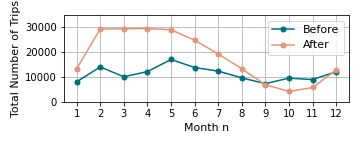
\includegraphics{ridesFigure.png}
  \caption{Comparison of Number of Cycle Hire Trips Per Months Before and After Pandemic}
  \label{fds-project-template:fig:ridesFigure}
\end{figure}

\begin{figure}[ht!]
  \centering
  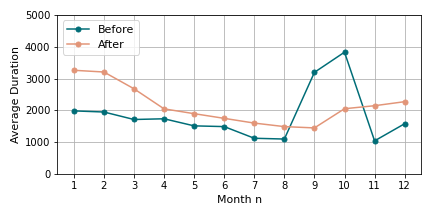
\includegraphics{durationFigure.png}
  \caption{Comparison of Average Cycle Hire Duration Per Month Before and After Pandemic}
  \label{fds-project-template:fig:durationFigure}
\end{figure}

Then, I visualised the number of rides per month with the cycle hire dataset. I plotted two lines in a line graph (Figure~\ref{fds-project-template:fig:ridesFigure}) to represent the number of rides before and after the pandemic. Through the graph, it is obvious that there are more rides after the pandemic, especially in the first six months after the pandemic. I also used A/B testing to give a more statistical answer, by implemented a bootstrap on before and after pandemic data tables, and took $B=10000$ bootstrap samples. For iteration $j$ in $1,...,B$, I re-sampled $n_{before}^*$ and $n_{after}^*$ for $n = 2000$ times from the corresponding datasets with replacement, then computed and stored difference $d_j^* = n_{before}^*/n - n_{after}^*/n$. Finally, I plotted the bootstrap distribution of $d^*$ (Figure~\ref{fds-project-template:fig:ab1}) and computed the desired quantiles and mean. Since it is a right-tailed CI, the 99\% CI is (-267.8,-211.2), and the mean is -234.0. Therefore, I proved that the number of rides after the pandemic is increased by an average of 234 times per day. I also plotted a graph for comparison of average ride duration before and after the pandemic (Figure~\ref{fds-project-template:fig:durationFigure}). It shows after the pandemic, the overall average duration increased as well, except in November and December 2019 there is a huge peak for unknown reasons. I implemented similar A/B testing on it and drew the distribution graph (Figure~\ref{fds-project-template:fig:ab2}), the 99\% CI is (-363.7,-134.5), and the mean is -220.4, which also proved that the average duration of rides after the pandemic is increased by a mean of 220.4 seconds.

\begin{figure}[ht!]
  \centering
  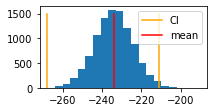
\includegraphics{ab1.png}
  \caption{Bootstrap simulation of A/B test on number of rides per day}
  \label{fds-project-template:fig:ab1}
\end{figure}

\begin{figure}[ht!]
  \centering
  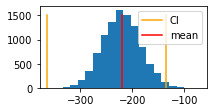
\includegraphics{ab2.png}
  \caption{Bootstrap simulation of A/B test on average duration per day}
  \label{fds-project-template:fig:ab2}
\end{figure}

The reason for this fact may be that in the early period of the outbreak, many citizens chose to use bike-share due to fear of being infected on public transport. After August 2020, as the epidemic became stabilised and more anti-epidemic measures were implemented, people began to take public transport again, which led to a decline in the average duration and number of people using bike-share. Since November, the average duration and number of rides per month have basically fallen back to the normal level as before the pandemic.

I also visualised the change of popular routes before and after the pandemic (Figure~\ref{fds-project-template:fig:mapFigure}). Rides have the same or opposite start and end stations are regards as the same route, and I counted the appearance of each route. Then, I sorted them and took the top 8 popular routes both from before and after the pandemic’s data tables. For each route, I plotted it on the same map with the given latitude and longitude, and got this graph. From this picture, we can see that after the epidemic, parks and beaches become the main destinations for people to ride bikes. Correspondingly, stations located in the downtown areas are no longer popular. This can reflect the change of people's cycling purpose. Now, more people cycle for leisure.

\begin{figure}[ht!]
  \centering
  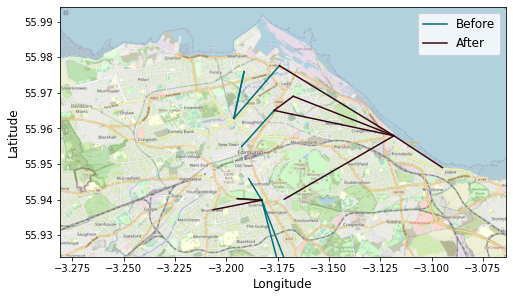
\includegraphics[scale=0.85]{mapFigure.png}
  \caption{Top 8 Popular Routes Before and After Pandemic}
  \label{fds-project-template:fig:mapFigure}
\end{figure}

\section{Discussion and conclusions}
% Suggested 400 words.

\paragraph{Summary of findings}

According to my analysis, there is a moderate negative correlation between the number of trips per day and new incremental infected cases on that day. The number of rides and average duration after the pandemic is larger than before. Moreover, more people cycling for leisure, instead of commuting during the pandemic, as the popular routes changed and stations near Portobello Beach and the Meadows now become popular.

\paragraph{Evaluation of own work: strengths and limitations}

In my opinion, there are several strengths in my work. First, I used visualisations to answer the last two questions clearly. When comparing the usage of bike-share before and after the epidemic, I used a line graph to visually compare the numbers. When exploring the changes of popular stations and routes before and after the epidemic, I marked the popular routes with different colours on a map, so I can see the location of the popular stations before and after the epidemic intuitively. However, there are still some limitations to my project. When comparing the usage of bike-share before and after the epidemic, the data are likely to be influenced by other factors such as weather and popularity of cycle hire, which makes the conclusion less reliable. In addition, it might be more intuitive to use a heat map to show the popularity of stations.

\paragraph{Comparison with any other related work}

City Monitor’s media article also demonstrated similar conclusions that the effect on the usage of bike-share is much less than the effect on public transport. Besides, parks and other outdoor recreation spaces topped the list of where people were travelling. The conclusion in BBC’s media report shows bike sale is increased a lot, which also support the fact that the usage of bike-share is rising.

%E.g. ``Anscombe has also demonstrated that many patterns of data can
%have the same correlation coefficient'' \cite{Ansc73Grap}.

%Wikipedia can also be cited but it is better if you find the orginal
%reference it for a particular claim in the list of references on the
%Wikipedia page, read it, and cite it.

%The golden rule is always to cite information that has come from other
%sources, to avoid plagarism \cite{wiki:plagarism}.

\paragraph{Improvements and extensions}
I think an improvement that can be made is to find a better variable to represent the severity of the epidemic when calculating the correlation between bike-share usage and the severity of the epidemic. This is because the daily new case can be effected by many factors like the number of Covid-19 tests, and it cannot precisely represent the severity on that day. Another improvement I want to do is to classify the stations into some categories, like commuting, leisure, home, business. Every station will be assigned to one label which can best describe itself. By analysing the change of the proportion of each type in 50 most popular stations, we can see the change of trend about what people cycling for. It is easier to understand and more convince for readers, compare to the current method which is plotting them on a map. 

A good extension is to find out the association between bike-share usage and other factors like seasons, weather and temperature. Such analysis can give us a better understanding of how bike-share usage is affected by other factors and provides the possibility of estimating future changes in bike-share usage, which is helpful for operating the cycle hire scheme in the future.

\bibliographystyle{unsrt}
\bibliography{fds-project}
\end{document}
